\documentclass[letterpaper, 12pt]{article}
\usepackage{palatino}
\usepackage{graphicx}
\usepackage{amsmath}
\usepackage[margin=1.5cm,includefoot]{geometry}
\usepackage{multicol}
\usepackage[mathscr]{eucal}
\usepackage{wrapfig}

\title{Thirdmode Store Administrator Guide}
\author{Michael Schmitz\\
        Thirdmode Web Projects
}
\date{\today}
\begin{document}

\maketitle
% \begin{multicols}{2}

\tableofcontents

\section{Introduction}
The {\em Thirdmode Store, or TMS for short,} is a web site construction framework for medium or large commercial web sites.  Like all online stores there are actually two web sites, the customer web site, and the administrative web site.  The customer web site presents products, methods to navigate, search, sort, and filter search results, a shopping cart, a login and password recovery process, a checkout and payment process, and an order status view.  The administrative web site is designed so that after an intial setup phase (that may involve a programmer and a CSS designer), a merchant with little or no technical experience can take over the ongoing maintenance.   The merchant can define categories, navigation tabs, product families, product attributes, and products and edit these objects and their relationships.  These operations can target large numbers of objects at once, so tedious one-at-a-time operations are avoided.  Further, these operations enforce logical and systematic organization of the objects.  Finally, the results of these operations are immediately visible on the customer web site.

There is also basic support for back-office procedures.  Through PayPal Pro, authorization, full or partial capture, voiding an authorization, full or partial refund of a sale, reauthorization, and ayschronous notifications are all supported.  The merchant can view all orders and sort them in various ways, or select only those that are in ``OK to Ship'' status.  Email alerts can be set up for customer initiated disputes, inventory-low warnings and so forth.  TMS is also integrated with UPS, so that exact shipping options and costs can be presented to the customer during the checkout process.  PayPal standard is also supported, and there is also some support for the Braintree payment gateway.

TMS is delivered as a {\em Ruby on Rails} application.  The setup phase can become very involved depending on the merchant requirements.  Perhaps integration with an existing Oracle (or non-Oracle) database is required, perhaps the merchant wants to use an Oracle RAC cluster, perhaps use of Oracle {\em In-Memory Database Cache (IMDB)} is appropriate.  The standard deployment uses the Apache Web Server, the Phusion Passenger module for Apache, and Oracle 10g or higher.

There are many companies that provide tools to build an online store,  {\em Yahoo! Stores}, or {\em Shopify} are examples.  TMS differs from these stores in several ways:
\begin{description}
 \item[Scalability]  TMS is designed to support a handful of products up to a million products in a scalable manner.  The scalability applies to both the customer who purchases items on the web site, as well as to the merchant who sets up and manages the site. 
\item[Performance] Keyword or description searches, product filtering, and navigation are all optimized by the use stored procedures in the Oracle database.  
\item[Bulk Operations] Although a TMS may have thousands of categories and a million products, administrative operations are provided that can affect large subtrees of categories.  For example, any subtree of the category tree can be easily reparented, renamed, deleted and so forth.  All the affected database tables will be automatically updated.  
\item[Payment Processing] Payment processing is currently supported through the PayPal and BrainTree payment gateways.  Final sales, authorization, full or partial capture, void of authorization, and refund are all supported.  
\item[Back Office Support] An asynchronous daemon listens for notifications from the gateways.  These notifications include transaction completions and reversals due to customer disputes.  The merchant (or administrator) can view a table of Orders that can be sorted in several ways, for example, orders that have been approved but not yet shipped.  He or she can edit the table to reflect the current state of the order.
If a product is given a ``low inventory'' theshold, TMS can be configured to send email to the merchant when the stock on hand drops below this threshold.
\item[Oracle Scalability] Because  TMS uses the Oracle Database, scalability via RAC clustering and/or Oracle TimesTen can be used to improve scalability. 
\item[Oracle Apps] Integration with other Oracle products such as Oracle Financials is possible.  This is optional, since TM does provide usable and effective back-office support on its own.
\item[Product Filters] Product ``filters'' that may be shown in the context of any category are automatically generated, based on all the filters that apply for all the products that are associated with the category.   This would be laborious and error-prone to do by hand.  In addition, the filters are maintained correctly during bulk operations.
\item[Shipping Costs] The TMS can contact UPS directly to present shipping choices and rates to the customer.
\item[Breadcrumb Trail] A breadcrumb trail is always presented to the user.  It includes the path through the tree of categories, as well as any searches that have been performed or filters that have been applied.  The customer can click on any element of the trail to go back to the view represented by that element.
\item[Open Source] TMS is open source and is built on the ``Ruby on Rails'' platform.
\end{description}

In this document, the {\em merchant} is the owner of the web-site.  The merchant is responsible for setting up and maintaining the web-site.  Only the merchant has access to the administrative portion of the web-site.  When the store is intially set up, the merchant will typically need to hire a programmer to do specific customizations and a designer to beautify the web-site.  TMS is provided with bare-bones styling.  The intent is that after the store is set up in this way,  the on-going maintenance of the site can be done by the merchant: defining the category tree,
defining attributes, defining product families, adding attributes to product families,  adding products to product families, defining the attribute values for a product, rearranging the category tree, fulfilling orders and flagging them as ``shipped'', voiding authorizations and so forth. 

On the other hand, the {\em customer} actually navigates/searches the web-site and purchases products. 

This guide discusses how the merchant can set up and maintain the store.

\section{Definitions}
There are a few very important concepts that need to be understood to set up the store.

\subsection{Product}
{\em Products} represent the actual types of items that are for sale in the store.  Thus a product will typically have an SKU or a part number.
When a product is added to a {\em product family} it may be given a value for each {\em product attribute} in the product family.  Alternatively,
the product may be edited later, and the values modified or assigned.

\subsection{Category}
As in practically all web sites, navigation is done by traversing a tree-structured hierarchy of menus. The {\em category tree} defines this menu hierarchy. A category is best thought of as a \textit{navigation tab} rather than as a grouping of products.  As the customer navigates through the web site, he or she is always in the context of a category (the current category).  Only products in that category are visible to the customer. 

Interestingly, it is possible to build a TMS with no categories at all, except for the root category.  In this case, products can be searched and filtered, but there is no tree of products to navigate through. 

\subsection{Leaf Category}
A \emph{leaf} category is a category that has no subcategories. 

\subsection{Ancestor Category}
A category  $A$ is an \emph{ancestor} of category $B$ if the path from the root to $A$ includes $B$ and $B \neq A$. In particular, the root category is an ancestor of every category except itself.

\subsection{Product Family}
A {\em product family} is a container for a set of \textit{product attributes}. Every product belongs to exactly one product family.  The product family that the product belongs to determines the set of attributes that the product may have.  A product family may be associated with one or more leaf categories.

\subsection{Product Attribute}
A \textit{product attribute}, or simply \textit{attribute} defines some characteristic that products may have.   It is a self-contained concept.  It is not defined with respect to a product family, category, or product.  After it is defined, an attribute can be added to one or more product families.  (If a product family is like a database table, adding an attribute to a product family is like adding a column to the table.)

\subsection{Filters}
\textit{filters} are based on product attributes.  In fact, filtering is really an activity based on underlying product attribute information.  Filters are presented to the customer as a set of either \textit{enumerated choices} (for integer enum or string attributes) or \textit{ranges} (for currency, and integer attributes).  When the customer clicks on a choice or a range, only products having a value for that attribute that matches the choice or falls within the range are displayed.

\subsection{Visibility}
Assume that a category $C$ has a product family $F$ and that a product $P$ is in $F$.  That is not enough to make $P$ visible to the customer when he or she navigates to category $C$.  The product $P$ must also be configured to be {\em visible} in $C$.

\subsection{Display Priority}
A category may contain thousands of products.  These can not be shown to the customer all at once, although a paging facility is provided.  To support the idea of ``featured'' products or ``most popular'' products, the merchant can assign a priority to the product that determines how close to the first page the product is initally displayed.


\section{Consistency Rules}
\begin{enumerate}
\item A product family can be created as an independent entity.
\item A product attribute can be created as an independent entity.  
\item A given product attribute can be added to many product families.
\item A product attribute can be removed from a product family at any time.
\item A product can only be created with reference to a product family.
\item A product can be removed from a product family at any time.
\item A product always belongs to exactly one product family.
\item A product may (but is not required) to have a value for each attribute in the product family.
\item The anonymous top-level (or root) category always exists.
\item A product family may only be directly associated with a leaf category.
\item If a category has a product family, then all its ancestors also have the product family. 
\item The filters for a category are derived from the intersection of all the attributes in its product families.
\item A product may only be directly associated with a leaf category.
\item If a product is associated with a leaf category, then it is also associated with all the ancestor categories of the leaf.
\item A product may only be associated with a leaf category if it belongs to a product family associated with the leaf category.
\item A product will only be shown to the customer in the context of a category if the product is visible in the category.
\item Visibility may be eplicitly set only for products in leaf categories.
\item If a product is visible in a category, then it is visible in all the ancestor categories.
\end{enumerate}

\section{Overview of Store Initialization}

Assume that the store has already been set up, but that it is empty -- no products, no product families, etc.  What does the merchant actually do to set up the store?  There are many different order of operations that are possible.  The following is only an example.

\begin{enumerate}
\item Define the category tree.  This may be done by visiting the ``admin/categories'' URL.
\item Define one or more product families.  This may be done by visiting the ``admin/product\_families/new'' URL.  This page requires you to choose one or more leaf categories to associate with the new product family.
\item Define some attributes to add to your new product families.  This may be done by visiting the ``admin/product\_attributes/new'' URL.
On this page, choose at least a name, a globally unique name, and an attribute type. For an integer enum or string attribute fill in the discrete choices for the possible values of the attribute.  For a integer or currency attribute, the value fields represent the endpoints of the ranges (or intervals) that the user may filter on.  For example, if you enter 3, 10 100 in the first three numerically labeled fields, then you have defined intervals $[0, 3)$, $[3, 10)$, $[10, 100)$, and $[100, \infty)$.  Note that these intervals include the left endpoint but not the right.
\item Edit your product families to add some or all of the new attributes.  Visit the ``admin/product\_families'' URL and click on the name of the product family that you want to edit (add attributes to) from the left hand column of the table. You will see some information about the product family.  Click ``Edit Product Family'' to perform the edit.
\item Add your product family to one or more leaf categories.
\item You are now on the edit page for a particular product family.  On this page you can change any information about the product family, view the attributes already in the product family, and search for, add, or delete other attributes.
\item Next visit the products page by clicking on the ``products'' link.  First choose a product family for the product from the list in the left sidebar.  You will see a form to fill in attribute values (for the chosen product family) for this product.  Do this an click submit.  You will be returned to the same page.
\item Still on the ``edit product'' page you will see some choices for visibility paths.  These correspond to the leaf categories where the product family for this product is associated.  Select one or more of these paths and click submit.  Then the product will be visible in all the selected leaf categories and all ancestors.  You will be returned to the same page.
\item Still on the ``edit product'' page, you may upload photos.  These may be thumbnails, gallery photos, or full size.  By clicking on the ``edit photos'' link you can indicate which full size photo corresponds to which gallery photo.  
\end{enumerate}


\begin{center}
\begin{figure*}
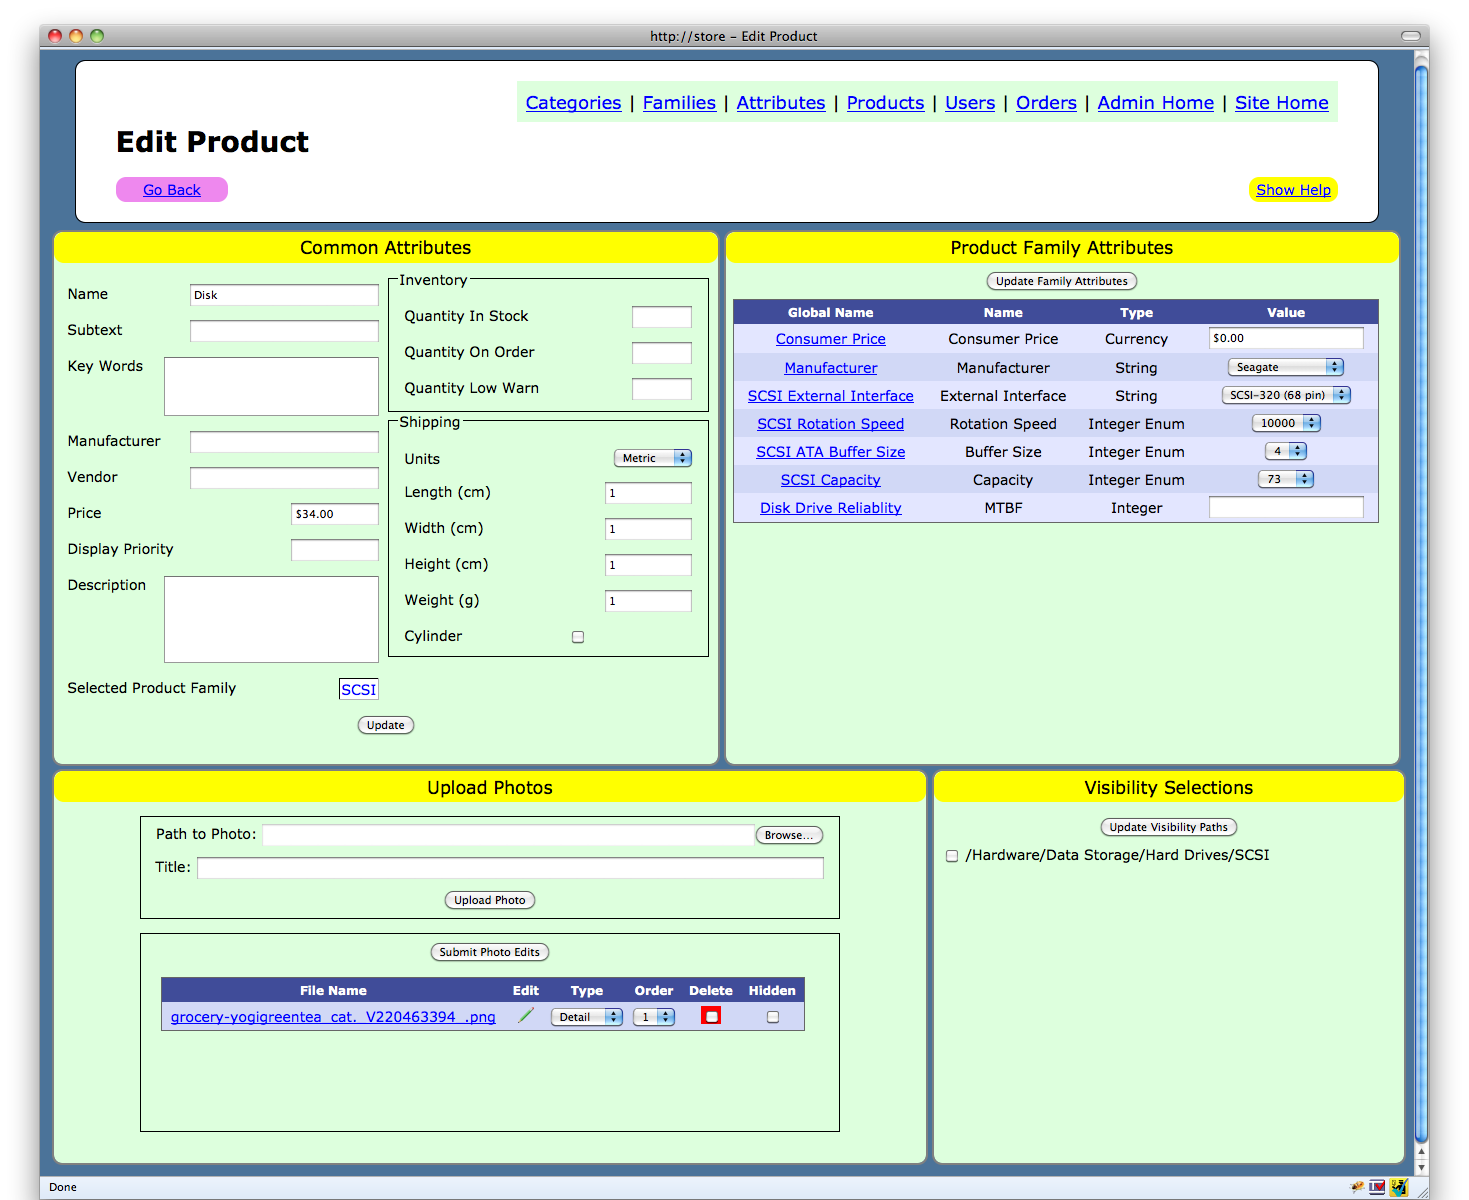
\includegraphics[scale=0.35]{product-edit}
\caption{\label{product-edit}Edit Product Page}
\end{figure*}
\end{center}

\section{Product Family}
For example, we may have a product family called {\em Cameras} with attributes {\em Is\_Digital}, {\em Brand}, {\em Megapixels}, {\em Price}, {\em Optical\_Zoom}, {\em Condition}, {\em Avg\_Customer\_Review}, {\em View\_Finder\_Type}, {\em Display\_Size}, {\em Seller}, {\em Image\_Stabilization}, and {\em Auto\_Rewind}.  This product family is intended to include both digital and film cameras.  Note that not all the attributes are applicable to both types of cameras.

\section{Category}
 To avoid ambiguity, categories should may named by their full path in the hierarchy. I.e. \textit{/automotive/brakes/shoes} is a different category than \textit{/footwear/children/shoes}.



A product family must have a unique name, i.e. two product families can have the same name.

After a product family has been defined, products can be added to the product family.  In fact, when a product is first created, it must be assigned to a product family.  At that time (or later) values for that product can be assigned.  For example, if we create a product {\em Nikon N80} in the Cameras product family, we can assign the value \textit{false} to \textit{Is\_Digital}, the value \textit{true} to \textit{Auto\_Rewind},
but leave attributes that do not apply, such as \textit{Megapixels} blank.

A product is always assigned to exactly one product family.  It may help to think of a product family as a database table and the attributes of the product family as being the columns for that table.  Adding a product to a product family is like creating a row in this table.  [Note: this is not at all what the database schema is like!]

\subsection{Product Attributes}
A \textit{product attribute}, or simply \textit{attribute} defines some characteristic that products may have.   It is a self-contained concept.  It is not defined with respect to a product family, category, or product.  After it is defined, an attribute can be added to one or more product families.  (If a product family is like a database table, adding an attribute to a product family is like adding a column to the table.)

\subsubsection{Attribute Types}
Each product attribute has a type:
\begin{description}
\item[string] This is an enumerated  attribute.  The attribute defines its set of allowed values.  For example, a \textit{color} attribute may define values \textit{red}, \textit{green}, and \textit{blue}.
\item[integer] Any integer value $>= 0$ is allowed.
\item[integer enum] This is an enumerated attribute.  The attribute defines its set of allowed values.  For example, a \textit{rotation speed} attribute may define values \textit{7200} and \textit{15000}.
\item[currency] A price together with the currency type.
\end{description}

\subsubsection{Attribute Choices and Ranges}
In addition to having a type, an enumerated type defines
For the integer and currency attribute types, the \textit{ranges} is simply a set of contiguous intervals that partition $[0, \infty]$.

You can define the set of ranges or choices when the attribute is created, or you can edit the product attribute later.



\begin{wrapfigure}{R}{0.2\textwidth}
\begin{center}
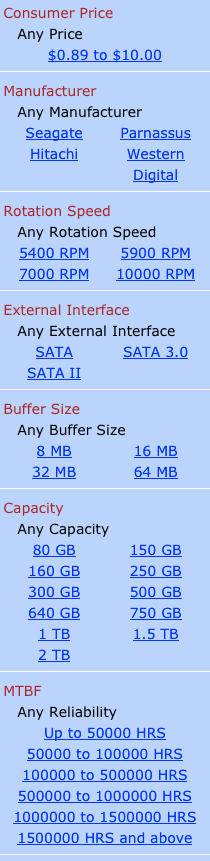
\includegraphics[scale=0.4]{attribute-sidebar}
\end{center}
\caption{Filter Sidebar}
\end{wrapfigure}

\section{Product Visibility}
Product families restrict where in the category tree that that its associated products can be displayed.  Specifically, a product family can be assigned to one or more leaf categories.  Then any products that belong to this product family are eligible to be displayed to the customer in this leaf category as well as all its ancestors.

Whether or not the product \textit{is} actually displayed depends on the product itself.  For example, suppose that there is a leaf category called \textit{Closeouts}, and that every product family is added to this category.  This makes every product \textit{eligible} to be displayed in the Closeout category.  (It also means that few or no filters will be available to the customer when viewing this category -- see below).  Any products that truly are closeout items should be added to this category individually.


\subsection{Displayable and Displayed Product}
Within the context of a category, only a subset of all possible products can be shown to the user.  Such products are called {\em displayable} products.  Typically, not all displayable products are shown or {\em displayed} to the user.  The displayable concept limits what can be displayed.

\subsection{Filtering on Attributes}
Within every category context, the search filters may be shown.  Each filter must ``make sense'' for all the displayable products in the category.  Filters are based on {\em attributes}: select a certain color, select a certain size, etc.

\subsection{Product Family}
Products that have similar attributes are grouped into a {\em product family}.  Each product belongs to exactly one product family.  Since a product family is associated with a set of attributes, all the products in a product family share the same set of attributes.  When a product family is associated with a leaf category, all its products become displayable in that leaf category as well as all its ancestors, all the way up to the root category.  A given product family can be associated with more than one leaf category, and a given leaf category may be associated with more than one product family.

\section{Breadcrumb Trail}
At any point, the user can see the current category context via a breadcrumb trail.  This is a representation of the path from the root category to the current category.  In addition, any search or filters that have been applied to the current view are appended to the path in the order that the choices have been made.  The user may click on any component of the trail to revert to any past view, including search or filter components. Any number of filters may be consecutively applied to a category context or after a search. However, starting a new search {\em after} filter choices have been made removes all filter choices from the path --- the user view reverts to the last category context followed by the new search.  This is done to prevent confusing the user.  The user may have trouble keeping track of the meaning of ``search after filter''.  On the other hand, ``filter after search'' does seem to make more intuitive sense.

\section{Displayable Products}
Here is how the displayable products for a category $C$ are determined.  Let $\mathscr{P}$ denote all product families that are associated with a leaf category that is a descendent of $C$.  The displayable products for $C$ are all the products that belong to some product family in $\mathscr{P}$.  This is abbreviated $displayable(C)$
\par
Why is such a complicated definition used?  It is primarily to support filtering on attributes.  The same attribute filters apply for all the products in a product family (since all these products necessarily have the same attributes).  If we take all the products from a number of product families, then we can only filter on the attributes that are in common to all these product families.  Thus, as the number of product families increases, the number of available attributes that we can filter on decreases.  Towards the leaf categories many specific filters can be used.  Towards the root, only very generic attributes can be used as filters, such as ``price''.
\par
In an interior category, the displayable products are all the products that ``bubble up'' from the product families defined at its leaf descendants, and the attributes that are available to filter on are  the attributes that are in common across all these product families.

\section{Categories}
As a customer traverses the store he/she is always in the context of some particular category.  On first visiting the site, the customer is in the context of the {\em root category}.   The initial set of products that the merchant wants the customer to see are displayed in this category.

Below the root category are the {\em top-level categories}.  These are the categories that appear in the {\em navigation bar} when the customer is in the context of the root category.  The top-level categories may have subcategories.  Categories up to four levels deep are supported.  (It is believed at this time that a deeper hierarchy of categories is not needed due to the search/filter capabilities that are provided.  If each category has ten subcategories, then there are 10,000 categories.  At 100 products per category, this supports 1,000,000 products. )

The category context determines the search and filter choices that are presented to the customer.

A category that has no descendants is called a {\em leaf} node.

The (unnamed) top-level category always exists, but the merchant may choose not to create any other categories.  In this case, there are no navigation tabs.  Products may be found using filters and searches as described below.  This is a certainly a viable approach when there are only a few hundred products.

At the other extreme, no filters need be defined.  Products could be found exclusively by searches or navigation through the category tree.

\begin{figure*}
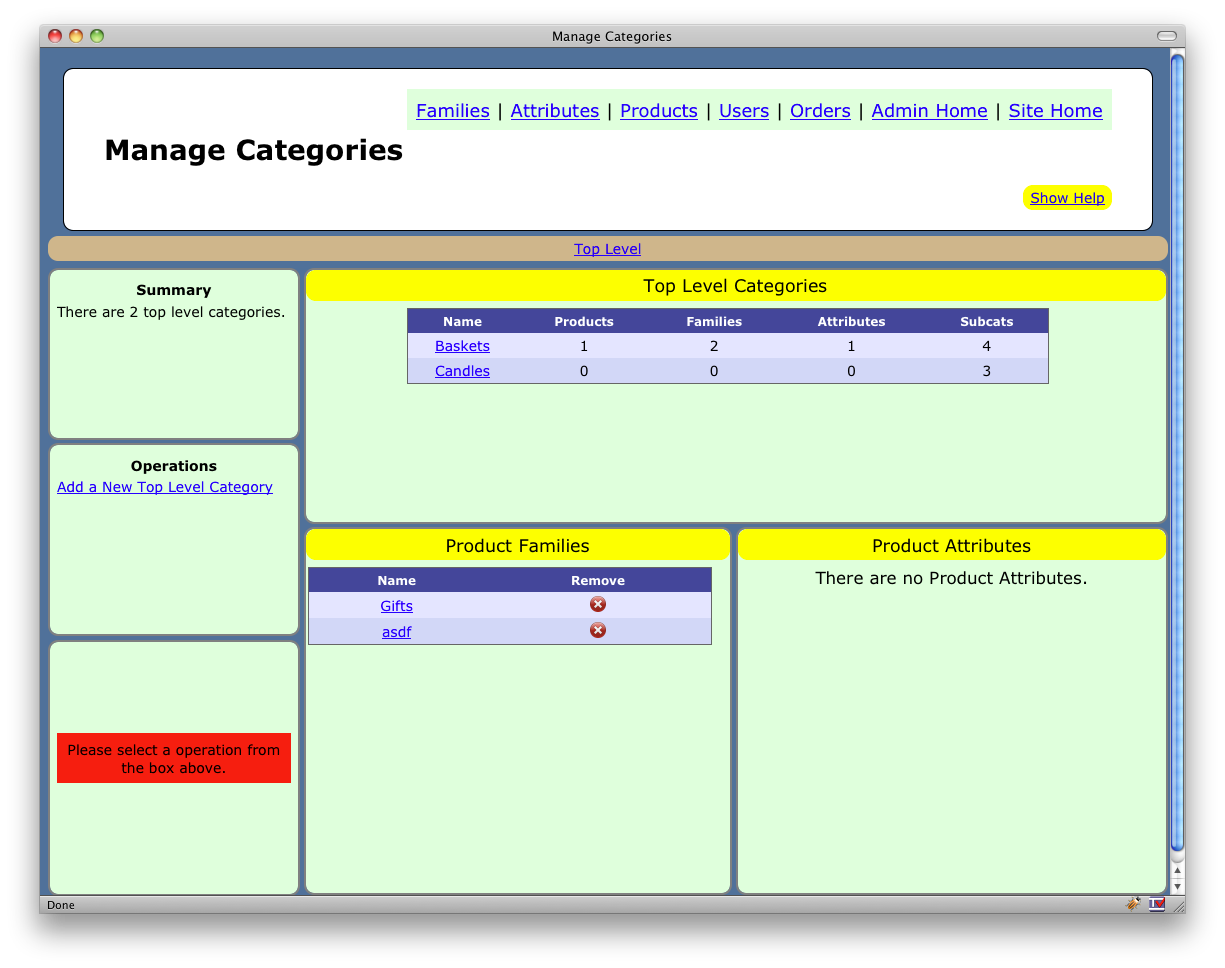
\includegraphics[scale=0.4]{categories-show}
\end{figure*}

\section{Displayed Products}
Just because a product is displayable in a certain category context doesn't mean it should be.  For example, all products are displayable at the root node.  Therefore, there must be a way to specify which products should be displayed in each category.  Further, it should be trivial for an administrator to set up and maintain.
\subsection{Importance Concept}
\par
For each pair $(prod, lcat)$ where $prod$ is a product, and $lcat$ is a leaf category that contains $prod$, there is an admistratively assigned $importance$ value. The $importance$ value controls how high up in the category tree the product is displayed along the path from the root to $lcat$. The value of $importance$ ranges from~$0$ to the length of this path.  (Note that a path with one node is considered to have length~$0$).  The value of $importance$ tells how many categories to omit (starting from the root) of this path before we start displaying the product. With this definition, a product is always displayed in $lcat$, and that if $importance$ is~$0$ then the product is displayed in all the categories in the path from the root to $lcat$.
\par
Since a product family can be associated to more than one leaf category, a product in this product family may be displayed in categories along more than one path.  It can have a different $importance$ for each path.
\par
\subsubsection{Administration for Product Creation}
When a product is created the admin must specify its product family. Once the product family is known, there are two further steps:  (a) attribute values can be filled in, and (b) the leaf categories (that are associated with the product family for the product) can be presented for the user to fill in the $importance$ value.

\subsubsection{Implementation Note}
A join table called $displayables$ can be used between the $products$ and $categories$ tables to hold the importance value.  This table links leaf categories and products and the table itself holds the $importance$ value.
\par
Another join table called the $product\_categories$ table, (that can be automatically regenerated from the other tables) will be used to hold the explicit many-to-many relationships between products and categories.
\par
What is the algorithm to generate the $product\_categories$ table?  Loop over the $displayables$ table --- for each triple $(P, L, I)$, get the path from leaf category $L$ to root, remove the first $I$ categories from the path to get a set of categories $\mathscr{C}$.  For each $C$ in $\mathscr{C}$ add the pair $(P, C)$ to the $product\_categories$ table.
\par This algorithm will be very slow.  Fortunately, there is never a need to do this, although the code base contains a function that implements this algorithm.

\section{Searches}
When a search is conducted within the context of a category, the search results are taken from the displayable products (not the displayed products.)  Thus a search may reveal products that were previously hidden within the category.  Note that this won't happen for a leaf category.  All the displayable products are always displayed at a leaf category.

\section{Operations on the Category Tree}
To make management of the store as flexible and convenient as possible the tree of categories may be modified with the following operations.
\subsection{Create}
Add a new category as a child of any category in the tree.  A category is automatically created as a {\em leaf} node.  This means it may have product families assigned to it.  If the parent category is a leaf category, any product families it has are moved to the newly created child. The parent becomes a non-leaf category.
\subsection{Delete}
Delete a category from the tree. Any category may be deleted at any time.  If the category has descendants, then the descendants become children of the category's parent node.  If a leaf category is being deleted and it has associated product families, then those product families may become orphans --- they are not associated with any leaf category.  Products in an orphan product family are not viewable in any category.
\par
If a leaf category is being deleted, all references to the leaf category should be removed from the $displayables$ table and the $product\_categories$ table.
\par
If an internal category $C$ is being deleted, then for all leaf descendants of $C$, if the depth in the category tree of $C$ is strictly less than the $importance$ of the leaf node, then decrement the $importance$ by $1$, otherwise leave it unchanged.  In the $product\_categories$ table, simply remove al rows that reference the category being deleted.

\subsection{Reparent}
To reparent a category means to move it and all its descendants to be a child of a different parent category.  In this case, the $product\_categories$ table does not need to be touched.  In the $displayables$ table, let $C$ denoted the category at the root of the sub-tree being moved.  If the depth of $C$ does not change, then nothing needs to be done.  Otherwise, add new\_depth - old\_depth to the $importance$ value of $importance$ for all products in all product families at the leaves of the subtree.

\section{Operations on a Category}
\subsection{Rename}
\subsection{Add Product Family}
\subsection{Remove Product Family}

\section{Database Schema}
It is helpful to understand the part of the database schema that relates to how the store is configured.  The most important tables are $products$, $product\_attributes$, $product\_families$, and $categories$.  In Figure~\ref{schema02}, these tables are denoted by the corresponding model names in Rails.  For example, the $products$ table in the database corresponds to a model named Product.  An arrow indicates a \emph{belongs-to} relationship.  For example, the arrow from Product to ProductFamily indicates that each Product belongs to exactly one ProductFamily.  There are four join tables in the schema.  In the figure, these have a red background.  These are used to handle many-to-many relationships.  For example, one Product can have many Categories, and one Category can have many Products.  
\par
The $category\_attributes$ table may be completely computed from the other tables.  It exists to make some database queries more efficient.  It answers the question: ``Given a Category, what are all the ProductAttributes that are in common to all the Products that may be in the Category?''  At the other extreme, the $family\_attributes$ table is completely specified by the admistrator as the store is built or maintained.  It is modified as the administrator adds or removes ProductAttributes from a ProductFamily.  The remaining two join tables $category\_products$ and $category\_families$ are hybrids, they are partly specified and partly computed.  The $category\_products$ table is used to answer this question: ``Given a Category, what are all the Products in the Category?''.  Similarly, the $category\_familes$ table is used to answer the question: ``Given a Category, what are all the ProductFamilies in the Category?''.  


\begin{figure*}
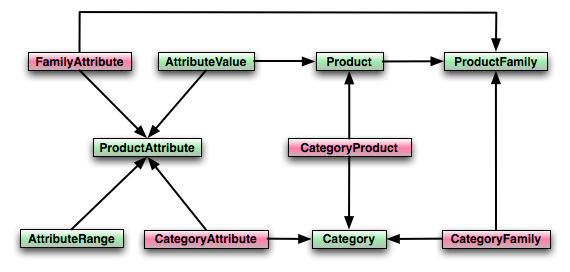
\includegraphics[scale=0.9]{schema}
\caption{\label{schema02}Database Schema}
\end{figure*}


% \end{multicols}
\end{document}

